\documentclass[10pt, conference, letterpaper]{IEEEtran}

\ifCLASSINFOpdf
	\usepackage[pdftex]{graphicx}
	\graphicspath{{./figures/}}
\else
  \usepackage[dvips]{graphicx}
  \graphicspath{{./figures/}}
\fi
	
\usepackage[cmex10]{amsmath}
\usepackage[caption = false, font = footnotesize]{subfig}
\usepackage{amsthm}
\usepackage{amsfonts}

\newtheorem{theorem}{Theorem}
\newtheorem{lemma}{Lemma}
\newcommand*{\Rom}[1]{\uppercase\expandafter{\romannumeral #1\relax}} % new command to type upper case Roman numbers
%\usepackage[normlem]{ulem}
%\usepackage{algoithm}
%\usepackage{algpseudocode}
\usepackage{textcomp}
\usepackage{gensymb} % include degree mark


\DeclareMathOperator*{\argmax}{arg\,max}
\DeclareMathOperator*{\unif}{unif}
\DeclareMathOperator*{\E}{\mathrm{E}}
\DeclareMathOperator*{\LOS}{\mathrm{LOS}}
\DeclareMathOperator*{\NLOS}{\mathrm{NLOS}}
%\newcommand*\conj[1]{\bar{#1}}
%\newcommand*\mean[1]{\bar{#1}}
\newcommand{\overbar}[1]{\mkern 1.5mu\overline{\mkern-1.5mu#1\mkern-1.5mu}\mkern 1.5mu}


\begin{document}
\title{Indoor mmWave Wearable Networks: Analysis of Interference and MAC Scheduling}

\author{\IEEEauthorblockN{Yicong Wang and Gustavo de Veciana}
\IEEEauthorblockA{Department of Electrical and Computer Engineering, The University of Texas at Austin\\Email: yicong.wang@utexas.edu, gustavo@ece.utexas.edu }
}

\maketitle

\begin{abstract}

%Millimeter wave serves as an ideal solution for short range high bandwidth applications in wearable networks.
%The dense indoor wearable network poses challenges to the design of MAC protocols: different propagation of mmWave; large density of devices and user dynamics; heterogeneity in transmission capabilities and QoS requirements of devices.
In this paper, we study the interference between users and MAC scheduling for dense indoor mmWave wearable networks.
We first study the characteristics (number, location and sensitivity to motion) of ``strong interferers'', i.e., interferers a MAC protocol need to schedule, of a typical receiver in a dense environment.
Results show the number of strong interferers remains roughly constant as user density increases, and the ``worst case'', e.g., highest number of interferers and most sensitivity to motion, corresponds to intermediate densities.
We then revisit the current MAC design leveraging clustering and hierarchy, and study the relationship between cluster size and network performance. 
Results show that large clusters mitigate inter-cluster interference but provide less resource reuse while
Highly directional transmissions benefit more from smaller clusters. 
Furthermore, analysis results indicate that optimal cluster size and resource allocated to each user almost remains the same for high user densities.



\end{abstract}
\IEEEpeerreviewmaketitle

\section{Introduction}\label{section:introduction}
% 1. Motivation
The market for wearable devices is growing fast in recent years \cite{wearable} and research on wearable networks is now being actively pursued. 
In the future, users may be equipped with multiple interconnected devices on the body, some of which may require high bandwidths, e.g., augmented reality devices. 
To support the high data rates and high user densities, millimeter wave communication has been proposed as a possible solution and standards have been developed for short-range wireless personal area network (WPAN) in the mmWave band, e.g., 802.11ad \cite{80211ad}, 802.15.3c \cite{802153c} and ECMA387 \cite{ECMA387}.

% 2. Challenges
Dense wearable networks on mmWave band prensent new challenges on the design of medium access control (MAC) protocols due to different channel characteristics and network scenario. 

The propagation of mmWave is different from other bands in nature. 
The path loss (PL) in mmWave band is higher thus the transmission range is short. 
MmWave transmissions experience higher loss due to blockage and the loss in reflection is also high, which makes the channel depend mostly on line-of-sight (LOS) channels or major reflected non-line-of-sight (NLOS) channels.
Human body introduces a path loss of over 20dB \cite{humanshadowing} thus movements of user and neighbors may greatly change the channel.
Devices on mmWave band usually use directional transmission and reception, thus the antenna gain is non-uniform. As a result, the channels in mmWave band are sensitive to environments and motions. 
However, these characteristics may not be a bad thing, e.g., short range, directionality and blockage can reduce the interference seen by receivers, affiliating the interference management. 

Dense indoor environment means possibly very high user densities and dynamics, e.g., a crowded train cart, and the MAC protocol need to work in such environments.
The number of interferers can be high and the set of interferers changes over time due to user dynamics. 
It is an open question how much overheads are required to coordinate interferers and handle user dynamics in such environments.

Another key characteristic of mmWave wearable network is the heterogeneity of devices. 
Wearable devices may have different transmission capabilities in terms of beamforming/directionality, computation associated with transmission, transmit power and energy, etc. 
Furthermore, the traffic patterns of users are different, some users may require highly directional link between smart phone and augmented reality device while some other users have multiple low-directional devices. 
The heterogeneity makes it challenging to optimize MAC protocols and guaranteeing Quality-of-Service (QoS). 

The above characteristics affect the MAC design in different ways. 
The nature of mmWave propagation makes it possible to achieve higher spatial reuse, but scheduling users is challenging as the signaling can be unreliable and the interference relationship may change frequently. 
The high density of users and user dynamics in indoor environment suggests that the MAC protocol should coordinate with users with limited signaling to reduce overhead. 
The heterogeneity of devices requires between different transmissions be treated differently in MAC and the MAC should adapt to different devices and QoS requirements.

\emph{Contributions of the paper}
We review the nature of mmWave propagation for high density wearable networks to better understand the role of interference and the need for coordination and MAC scheduling in such environments. 
Our primary goal is to study the characteristics, i.e., number, location and sensitivity to motion, of the ``strong interferers'' as seen by a typical receiver in a dense wearable environment. 
The strong interferers are those that has a strong channel to a user and in principle a MAC protocol would aim to address through scheduling. 
Work has been done on analyzing the SINR distribution in dense wearable networks but they mostly assume there is no scheduling or simple protocols like Aloha \cite{interferencefinitesized}\cite{enclosedmmwave}.

Our main findings of interference environment include: 
\begin{itemize}
	\item The number of strong interferers does keep increasing with user density. 
	The average number reaches a peak then starts decreasing due to human body blockage. 
	\item In highly dense environment, most strong interferers are actually close by as the close neighbors around the user form a blocking ``ring'' round the user and block more distant interferers. 
	\item Strong interferers that are close by are less sensitive to users' local motions than those that are further away. 
\end{itemize}

Our results suggest in dense wearable network, the near neighbors are those that we need to coordinate to mitigate interference.  
The number of near neighbors is limited, thus the coordination overheads will be scalable, i.e., different user densities may require the same amount of signaling overhead. 
The ``worst case'', e.g., where users see highest number of interferers and most sensitivity to motion, do not necessarily correspond to scenarios with the higher user density due to blockage.

We then revisit current approaches to MAC design for wearable networks which leverage clustering and hierarchical scheduling. 
Our goal here is to study the relationship between cluster size and network performance in high density scenarios given the particular characteristics of mmWave propagation discussed above. 

Our main findings with clustering include:
\begin{itemize}
	\item The trade-offs associated with cluster size: large clusters reduce inter-cluster interference but requires more overheads and provide less reuse than small clusters.
	\item Heterogeneity of device transmission capabilities impacts the best cluster size: highly directional transmissions requires smaller cluster size while low directional transmissions require larger clusters to mitigate interference. 
	\item The best cluster size does not change with user density when user density is high and the resource allocated to each user may not decrease with density. 
\end{itemize}

Our results suggest that the cluster size is not sensitive to user densities, but need to adapt to changes in device transmission capabilities and traffic patterns. Clustering might be most challenging in intermediate dense scenarios.

\emph{Related work}
% Channel Modeling
The authors in \cite{urbanblockage} analyze blockage effects in urban areas and model penetration loss of the paths using stochastic geometry. 
The work in \cite{interferencefinitesized} studies human shadowing effects in finite-sized areas when users' locations are fixed. 
The authors use different path loss exponents and fading models to model the line-of-sight (LOS) and non-line-of-sight (NLOS) channels and approximately compute the signal-to-interference-ratio (SINR) distribution. 
Subsequently the authors in \cite{enclosedmmwave} model the SINR in random networks in an enclosed environment and incorporate the first order reflections off the walls, the ceiling and the floor. 
The analysis of the interference in the mmWave band has mainly focused on the distribution of SINR where users are uncoordinated, i.e., users  either all transmit or use simple MAC protocols like Aloha, where users transmit with a given probability. 
\cite{humanactivity}\cite{timevaryingpathshadowing}\cite{blockagein60ghz}study the impact of human mobility on fixed channels through measurements and simulation, but how the set of interferers is influenced is still unknown.

In dense wearable networks, the MAC protocol needs to coordinate the devices on different users to improve the reuse of the resources and ensure application QoS. 
The authors of \cite{dtdmac}\cite{mdmac} propose distributed MAC protocols for mmWave networks and use memory to improve the resource reuse of the system. 
\cite{onlinkscheduling} study the link scheduling for mmWave ad hoc networks with blockage.
The authors of \cite{intersharing} propose an inter-network spatial sharing strategy for 802.11ad to improve the resource reuse between multiple basic service sets (BSSs) by exchanging reports.
In dense wearable networks, the above MAC protocols may fail to coordinate amongst the users due to the large number of users or dynamic channels. 

\emph{Organization of the paper}
In the next section, We present the analysis of the number of strong interferers and their sensitivity to local motion in Section \ref{section:interference}. 
In Section \ref{section:clustering} we study the optimizing of clustering in hierarchical wearable MAC protocols.
We conclude the paper in Section \ref{section:conclusion}.

\section{Interference in Dense mmWave Wearable Networks}\label{section:interference}
In this section we try to characterize the interference environment a user would experience, i.e., the set of strong interferers.

\subsection{System Model for Wearable Network}\label{section:channel:model}
We consider a wearable network consisting of users standing on a 2-D plane.
Denote $x_i$ as the location of the center of user $i$. 
The devices on each user form a personal basic service set (PBSS), coordinated by the PBSS coordinate point (PCP), e.g., the smart phone of the user.
There is no access point (AP) or central controller coordinating or synchronizing users.
Walls and obstructions other than human bodies are not considered, and there is a ceiling at a height of $h_{\mathrm{ceiling}}$ meters. 

For simplicity, we assume the locations of PCPs on the human body are the same and the users' bodies are of the same dimensions. 
The height of users is $h_{\mathrm{body}}$ and the PCPs are located in front of user bodies at a height of $h_{\mathrm{device}}$.
A typical user is placed at $0$ with an orientation $\theta_0$. The locations of other users $\Phi=\{x_i\}_i$ follows a homogeneous Poisson Point Process (HPPP) with density $\lambda$.
The orientation of user $i$, $\theta_i$, are independently distributed in $[0, 2\pi]$.
The network is then modeled as an independent marked point process (i.m.p.p.) $\tilde{\Phi}=\{(x_i, \theta_i)\}_i$. 

We use the link between the centers of two users to approximate the actual channel between their PCPs. 
Only two channels are considered, the line-of-sight (LOS) channel and the reflected channel over the ceiling, denoted as the non-line-of-sight (NLOS) channel.
The path loss (PL) of LOS channel follows free space propagation and the reflection coefficient, $\Gamma$ is computed using the model in \cite{reflection}.
If a channel is blocked by human body, the PL is 0.
The PL between two users is approximated by the PL of LOS channel if the LOS channel presents, or the PL NLOS channel if the LOS channel is blocked. 

We consider the channel between two users from a MAC design perspective, i.e., whether the channel is strong enough that the two users can receive the signaling of each other.
Based on the above assumptions, the channel between $u_0$ and $u_x$ is strong if  
\begin{equation}\label{eq:PL_LOS}
|x| < r_{\max}
\end{equation}
for LOS channel, and 
\begin{equation}\label{eq:PL_NLOS}
|x| < r_{\max}^{\mathrm{reflection}}
\end{equation}
for reflected channel, where $|x|$ is the distance between $u_x$ and $u_0$, $r_{\max}$ is the max distance of a LOS strong interferer and $r_{\max}^{\mathrm{reflection}}$ is the maximum distance of a reflected strong interferer, which is related to $h_{\mathrm{ceiling}}$, $h_{\mathrm{device}}$ and the material of the ceiling. 

\subsection{Number of Strong Interferers}
In this section we analyze the number of strong interferers seen by a typical user, $N_{\mathrm{SI}}$. 
$N_{\mathrm{SI}}$ can be written as follows, 
\begin{equation}
N_{\mathrm{SI}}(\tilde{\Phi}, \theta_0) = \sum_{(x_i, \theta_i)\in \tilde{\Phi}}f_0(x_i, \theta_i, \tilde{\Phi}\backslash\{(x_i,\theta_i)\}, \theta_0)
\end{equation}
where $f_0(x_i, \theta_i, \tilde{\Phi}\backslash\{(x_i,\theta_i)\}, \theta_0)$ is the indicator function that $(x_i, \theta_i)$ is a strong interferer of the typical user $(0,\theta_0)$, if the two users faces each other, i.e., the channel is not blocked by self-blockage, and the channel satisfies the conditions in (\ref{eq:PL_LOS}) and (\ref{eq:PL_NLOS}).

$N_{\mathrm{SI}}$ depends on the realization of $\tilde{\Phi}$, making the distribution of $N_{\mathrm{SI}}$ hard to compute. 
Still the average number of strong interferers is a good metric to understand the coordination requirements of MAC.
Using the Reduced Campbell's formula for i.m.p.p. of Corollary 2.2 in \cite{stochasticgeometry}, we can compute $\E[N_{\mathrm{SI}}]$ in the following theorem,
\begin{theorem}\label{theorem:E_N_SI}
	$\tilde{\Phi}$ is an i.m.p.p., and $\mathrm{E}[N_{\mathrm{SI}}]$ is given by,
	\begin{equation} \label{eq:N_SI}
	\begin{split}
	\mathrm{E}[N_{\mathrm{SI}}] &= \mathrm{E}^0\bigg[\int\limits_{\mathbb{R}^2\times[0,2\pi)}f_0(x_i, \theta_i, \tilde{\Phi}\backslash\{(x_i,\theta_i)\}, \theta_0)\tilde{\Phi}(\mathrm{d}(x,\theta)) \bigg]\\
	&= \int\limits_{\mathbb{R}^2}\int\limits_{[0,2\pi)}\int\limits_{\mathbb{\tilde{M}}}\mathrm{E}_{\theta_0}[f_0(x,\theta,\tilde{\phi}, \theta_0)]P_{(x,\theta)}^{!}(\mathbb{d}\tilde{\phi})F_x(\mathrm{d}\theta)M(\mathrm{d}x).
	\end{split}
	\end{equation}	
\end{theorem}
In Theorem \ref{theorem:E_N_SI}, $\mathrm{E}^0$ is the expectation given that there is a user at the origin, $\mathrm{E}_{\theta_0}$ is the expectation over $\theta_0$, $\mathbb{\tilde{M}}$ is the set of all possible realizations of $\tilde{\Phi}$, $P_{(x,\theta)}^!$ is the Palm distribution of marked point process given that there is a point $(x, \theta)$ and a point at the origin. $F_x(\mathrm{d}\theta)$ is the probability measure of the orientation of the user located at $x$ and $M(S)=\mathrm{E}[\Phi(S)]$ is the mean measure of the points $\Phi$.

A user $(x', \theta')$ blocks channel $x$ if meeting the following two conditions as illustrated in Fig. \ref{fig:Channel_enb}: 1) the projection of $x'$ on the line from $0$ to $x$, $s_x(x')$ lies on the channel, $s_x(x')\in [0,|x|]$; 2) the cross section of user body projection on $n_x$,  $D_x(x, \theta')$, covers the origin $0$, $0 \in D_x(x, \theta')$.

\begin{figure}
	\centering
	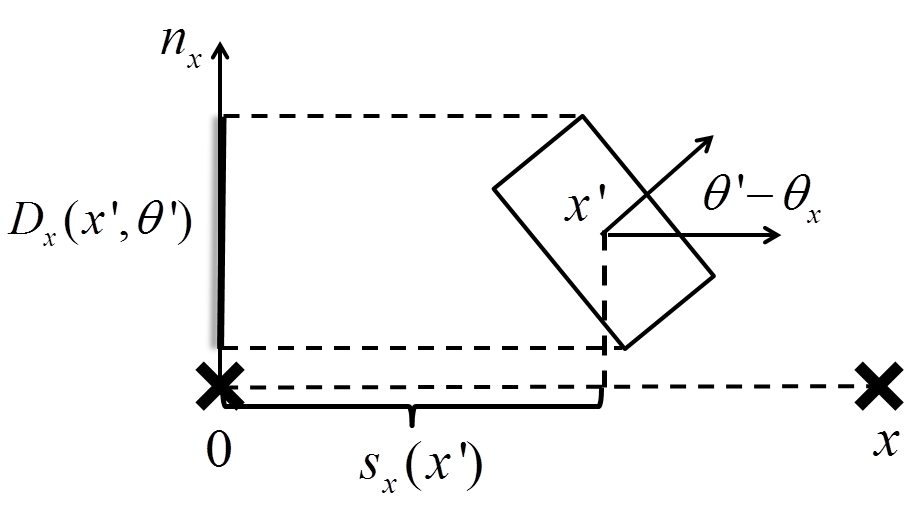
\includegraphics[width = 0.3\textwidth]{Channel_ENB.pdf}
	\caption{User $(x', \theta')$ will block the LOS channel between $0$ and $x$ if the projection of $x'$ lies on $x$ and the projection of his cross-segment covers $0$. }
	\label{fig:Channel_enb}
\end{figure}

The probability that a user located at $x$ is a LOS strong interferer of the typical user can then be computed in the following theorem.

\begin{theorem}\label{theorem:E_N_B_LOS}
	The number of users blocking the LOS channel between $0$ and $x$, $N_\mathrm{B}^\mathrm{LOS}(x)$, follows Poisson distribution and the average number of blockage $\mathrm{E}[N_{\mathrm{B}}^\mathrm{LOS}(x)] \approx \lambda |x| \mathrm{E}[D]$. $\mathrm{E}[D]$ is the expected width of cross section of user.  
\end{theorem}
\begin{proof}
	The number of blockages is given by,
	\begin{equation*}
	N_{\mathrm{B}}^\mathrm{LOS}(x) = \sum_{(x_i, \theta_i)\in \tilde{\Phi}\backslash(x,\theta)}1\big((x_i, \theta_i) \mathrm{~blocks~} l_{0,x}^{\mathrm{LOS}}\big).
	\end{equation*}
	$\tilde{\Phi}\backslash(x,\theta)$ is an i.m.p.p. and $1\big((x_i, \theta_i) \mathrm{~blocks~} l_{0,x}^{\mathrm{LOS}}\big)$ only depends on $(x_i, \theta_i)$. $N_{\mathrm{B}}(x)$ is an independently thinned Poisson process, which is still a Poisson process \cite{stochasticgeometry}. 
	
	\begin{align}
	\mathrm{E}[N_{\mathrm{B}}^\mathrm{LOS}(x)] & =  \int\limits_{\mathbb{R}^2}\int\limits_{[0,2\pi)}\mathrm{1}((x',\theta')\mathrm{~blocks~}(x,\theta))F_{\theta'}(\mathrm{d}\theta')\lambda(\mathrm{d}x') \nonumber\\
	& \stackrel{(a)}{\approx} \int\limits_{\mathbb{R}^2}\int\limits_{[0,2\pi)}\mathrm{1}\big(0\notin D_x(x',\theta')\big) \nonumber\\
	& \phantom{{}=1} \times \mathrm{1}\big(s_{x}(x')\in[0,|x|]\big) F_{\theta'}(\mathrm{d}\theta')\lambda(\mathrm{d}x') \label{eq:2dblocking} \\
	& \stackrel{(b)} = \lambda|x|\int\limits_{[0,2\pi)}|D_x(\cdot, \theta')| F_{\theta'}(\mathrm{d}\theta') \nonumber\\
	& \stackrel{(c)} = \lambda|x|\mathrm{E}[|D_x|] \label{eq:N_blockage_original}
	\end{align}
	where in (a), we use the two conditions of projections to approximate $\mathrm{1}((x',\theta')\mathrm{~blocks~}(x,\theta))$. In (b), we use the fact that users follows HPPP with density $\lambda$. The location the dimensions of users are independent of the locations of users thus the distribution of $|D_x(x', \theta')|$ is independent of $x'$. In (c), $\mathrm{E}[|D_x|]$ is the expectation of $D_x$ over user orientations.
\end{proof}

By Theorem \ref{theorem:E_N_B_LOS}, the probability that the LOS channel is blocked is $e^{-\E[N_\mathrm{B}^\mathrm{LOS}(x)]}$. 

\begin{figure}
	\centering
	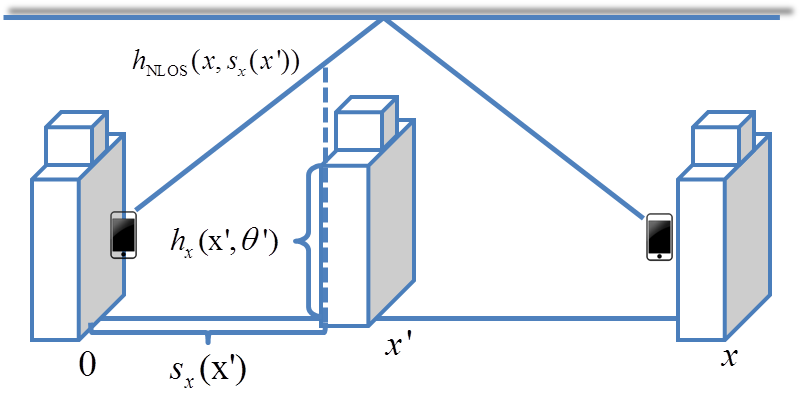
\includegraphics[width = 0.4\textwidth]{Channel_NLOS.pdf}
	\caption{User $x$ has a clear reflected channel if there is no other user blocking the reflection path, i.e., there is no user $(x',\theta')$ such that $\{s_x(x')\in [0, |x|]\}\cap\{ h_x(x', \theta') \geq h_{\mathrm{NLOS}}(x, s_x(x'))\}$.}
	\label{fig:NLOS}
\end{figure}

Similarly, we can compute the probability that the NLOS channel is not blocked by considering the height of blockage and NLOS channel as shown in Fig. \ref{fig:NLOS}. We assume that if the LOS channel is not blocked, then the reflected channel is clear but the LOS channel can be blocked if the reflected channel is clear. 

Combining the above ananlysis, $\E[N_{\mathrm{SI}}]$ is given by,
\begin{multline}\label{eq:E_N_SI}
\mathrm{E}[N_{\mathrm{SI}}] =  \int\limits_{\mathbb{R}^2}
\mathrm{P}_{\text{facing}}(x)\\
\cdot \big[\text{1}(|x|\in[r_{\min},r_{\text{max}}^{\mathrm{reflection}}])
\cdot e^{-\mathrm{E}[N_{\mathrm{B}}^\mathrm{NLOS}(x)]} \\
+ \text{1}(|x|\in[r_{\text{max}}^{\mathrm{reflection}},r_{\text{max}}])
\cdot e^{-\mathrm{E}[N_{\mathrm{B}}^\mathrm{LOS}(x)]} \big]\lambda(\mathrm{d}x),
\end{multline}
where $r_{\min}$ is the minimum distance between users, $P_{\text{facing}}$ is the probability that two users face each other,
\begin{equation*}
\mathrm{P}_{\text{facing}}(x) = \int\limits_{[0,2\pi)}\mathrm{E}_{\theta_0}[\text{1}((x,\theta)\mathrm{~faces~}(0,\theta_0))]F_{\theta}(\mathrm{d}\theta).
\end{equation*}

Fig. \ref{fig:channel:en_si} shows $\mathrm{E}[N_{\mathrm{SI}}]$ for different user densities and compare the analysis results with simulations. 
Users are modeled as cylinders with a diameter of 0.6m. 
To account for the fact that users can not overlap with each other, we use Mat\'ern \Rom{3} process \cite{matern} instead of HPPP to model the locations of users in the simulations.
Our analytical results are in line with the simulations, validating the accuracy of the approximation. 
$\mathrm{E}[N_{\mathrm{SI}}]$ first grows with the user density, but as user density further increases, it stops increasing.
Users see most strong interferers at moderately high user densities. 


\begin{figure}
	\centering
	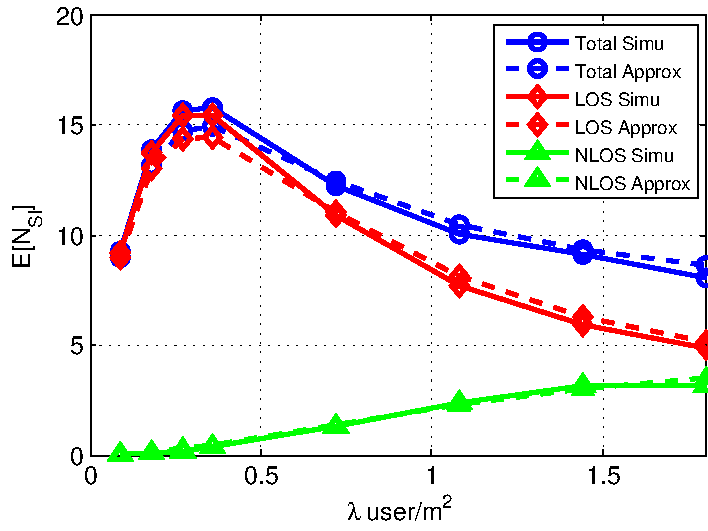
\includegraphics[width = 0.3\textwidth]{Channel_en_si.pdf}
	\caption{$\mathrm{E}[N_{\mathrm{SI}}]$ for different user densities. $h_{\mathrm{body}} = 1.754m$,  $h_{\mathrm{device}}= 1m$, $h_{\mathrm{ceiling}}=2.8m$. 
		The material of the ceiling is one layer polyester board with a thickness of 9 mm. 
		The threshold of path loss for strong interferers is -88 dB, $r_{\max} = 10\mathrm{~m}$, and $r_{\max}^{\mathrm{reflection}} = 3.1m$.}
	\label{fig:channel:en_si}
\end{figure}


\begin{figure}
	\centering
	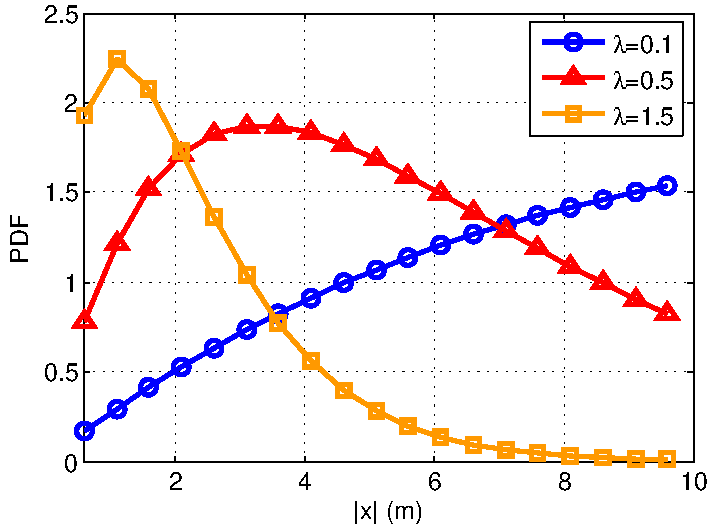
\includegraphics[width = 0.3\textwidth]{Channel_si_pdf.pdf}
	\caption{Probability density function of LOS strong interferers as a function of the distance to the typical user at $\bf{0}$.}
	\label{fig:Channel_si_pdf}
\end{figure}

\begin{figure}[htp]
	\centering
	\subfloat[$\lambda = 0.1/m^2$]{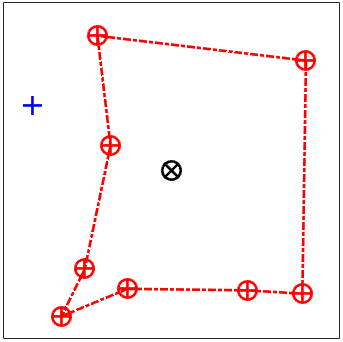
\includegraphics[width=0.15\textwidth]{Channel_jamming_01.pdf}} \hfill
	\subfloat[$\lambda = 0.5/m^2$]{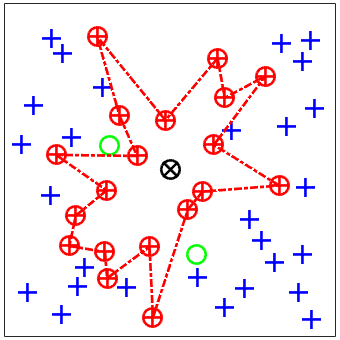
\includegraphics[width=0.15\textwidth]{Channel_jamming_05.pdf}} \hfill
	\subfloat[$\lambda = 1.5/m^2$]{\label{fig:channel:jamming} 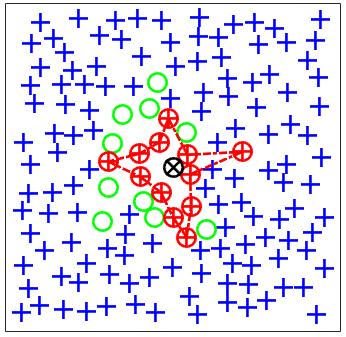
\includegraphics[width=0.15\textwidth]{Channel_jamming_15.pdf}}
	\label{fig:channel:variation}
	\caption{The locations of strong interferers for different densities, ignoring self blockages. Red circles represent LOS interferers, green circles are NLOS interferers and blue circles are not strong interferers.}
\end{figure}

Fig. \ref{fig:Channel_si_pdf} illustrates the distribution for the distance of strong interferers for varying user densities, with self blockage not considered. Fig. \ref{fig:channel:variation} shows the locations of strong interferers in one realization of the network.
As user density increases, the strong interferers tend to concentrate the receiver. When user density is very high, the network reaches a ``jamming regime'', where strong interferers are mostly close by and block further away interferers as shown in \subref{fig:channel:jamming}.
Such results indicate that it might be enough to coordinate close neighboring users.

\subsection{Sensitivity of Strong Interferers}\label{section:channel:sensitivity}
In this section we study the sensitivity of strong interferers to users' small local movements.
The sensitivity of strong interferers, i.e., how strong interferers changes when users move, influence the cost  and benefit of tracking and coordinating with neighbors.
 
Suppose in a time interval $[t, t+ \Delta t]$, users make translations and rotations, resulting in changes for the typical user and potential interferers summarized as follows:
\begin{equation*}
\begin{split}
(0,\theta_0)&\rightarrow(\Delta x_0, \theta_0 + \Delta\theta_0) \\
\tilde{\Phi}^{t}=\{(x_i, \theta_i)\}&\rightarrow\tilde{\Phi}^{t+\Delta t}=\{(x_i+\Delta x_i, \theta_i + \Delta\theta_i)\}
\end{split}
\end{equation*}

Let $Y_x^t=f_0(x, \theta, \tilde{\Phi}^t\backslash (x, \theta), \theta_0)$ be the state of the interferer located at $x$ at time $t$, and $Y_x^{t+\Delta t}$ be the state of the same user at $t+\Delta t$, which is given by,
\begin{multline*}
Y_{x}^{t+\Delta t} = f_{\Delta x_0}(x+\Delta x, \theta + \Delta\theta, \tilde{\Phi}^{t+\Delta t}\backslash (x+\Delta x, \theta + \Delta\theta), \\
\theta_0 + \Delta\theta_0),
\end{multline*}
$Y_x^t \mathrm{~and~} Y_{x}^{t+\Delta t} \in \{0,1\}$. $Y = 1$ if the user is a strong interferer of the typical user and $Y = 0$ otherwise. We define the sensitivity of an interferer originally located at $x$ for an interval of length $\Delta t$, $S(x, \Delta t)$, via the autocorrelation of the state of the interferer at $t$ and $t+\Delta t$, 
\begin{equation}
S(x, \Delta t)
=\mathrm{Corr}(Y_x^t, Y_x^{t+\Delta t})
=\frac{\mathrm{E}[Y_x^t\cdot Y_x^{t + \Delta t}]}{\sigma_{Y_x^t}\cdot \sigma_{Y_x^{t+\Delta t}}},
\end{equation}
$S(x, \Delta t)\in [0,1]$. If $S(x, \Delta t)$ is small, the autocorrelation between the states of the channel is small and the channel sensitive to movements; if $S(x, \Delta t)$ approximates $1$, the autocorrelation is high and the strong interferer is stable.

Based on our assumptions on $\tilde{\Phi}$ and independent movements, we have the following two theorems on the state of the network after user moves.

\begin{theorem}\label{theorem:hppp}
	If $\Phi^t$ is HPPP with density $\lambda$ and users make independent movements and the movements are independent of users' location, then $\Phi^{t+\Delta t}$ is still HPPP with density $\lambda$. 
\end{theorem} 
%\begin{proof}
%	Let $p_{t, t+\Delta t}(x, x+\Delta x)$ be the probability that the user located at $x$ at time $t$ moves to $x + \Delta x$ at time $t+\Delta t$. Users' movements are independent and the movements are independent of $x$, then $p_{t, t+\Delta t}(x, y)$ is a function of $\Delta x$, i.e., $p_{t, t+\Delta t}(x, x+\Delta x) = g_{t, t+\Delta t}(\Delta x)$.
%	According to the Displacement Theorem in \cite{poisson}, $\Phi^{t+\Delta t}$ is a HPPP with density $\lambda$.
%\end{proof}

\begin{theorem}\label{theorem:hppp_orientation}
	$\tilde{\Phi}^{t+\Delta t}$ is an i.m.p.p. and $\theta$ is uniform in $[0, 2\pi)$ at $t+ \Delta t$. 
\end{theorem}
%\begin{proof}
%	$\theta$ and $\Delta \theta$ are independent from other users and the locations and translations of users, $x$ and $\Delta x$, thus $\tilde{\Phi}^{t+\Delta t}$ is i.m.p.p.. If $\theta^t\sim \unif(0, 2\pi)$ and $\Delta \theta$ is independent from $\theta^t$, then follow the similar proof used in displacement theorem, $\theta^{t + \Delta t}\sim \unif(0, 2\pi)$. 
%\end{proof}

The proof of Theorem \ref{theorem:hppp} and \ref{theorem:hppp_orientation} are based on the Displacement Theorem in \cite{poisson} and uses the fact that $\Phi$ is HPPP and the orientations and movements of users are independent.

By Theorem \ref{theorem:hppp} and \ref{theorem:hppp_orientation}, $\tilde{\Phi}$ is stationary and the variance of $Y_x^t$ and $Y_x^{t+\Delta t}$ are the same and independent of $t$ or $\Delta t$ if we ignore the change in $|x|$, thus
\begin{equation*}
\mathrm{Var}(Y_x)=p_{\mathrm{SI}}(x)\cdot (1-p_{\mathrm{SI}}(x)),
\end{equation*}
where $p_{\mathrm{SI}}(x)=\mathrm{Pr}(f_0(x,\theta,\tilde{\Phi}\backslash\{(x_i,\theta_i)\}, \theta_0)=1)$. 

To compute $S(x, \Delta t)$, we further need $\mathrm{E}[Y_x^t\cdot Y_x^{t + \Delta t}]$, 
\begin{equation*}
\mathrm{E}[Y_x^t\cdot Y_x^{t + \Delta t}] = \mathrm{Pr}(\{Y_x^t=1\}\cap \{Y_x^{t+\Delta t}=1\}),
\end{equation*}
the probability that user at $x$ is strong interferer at $t$ and $t + \Delta t$. 
The movements of users during $\Delta t$, $(\Delta x, \Delta \theta)$ can be counted as the marks of $\Phi$, and we have a new m.p.p. $\tilde{\Phi}^{\Delta t} = \{(x_i, m_i)\}_i$, where $m_i = (\theta_i, \Delta x_i, \Delta \theta_i)$. According to our assumptions of independent movements, $\tilde{\Phi}^{\Delta t}$ is an i.m.p.p.. 

Denote $f_0^{\Delta  t}(x_i, m_i, \tilde{\Phi}^{\Delta t}\backslash (x_i, m_i), m_0)$ be the indicator function that the user located at $x$ is a strong interferer at $t$ and $t + \Delta t$, then 
\begin{multline*}
f_0^{\Delta  t}(x_i, m_i, \tilde{\Phi}^{\Delta t}\backslash (x_i, m_i), m_0) = \\
f_0(x,\theta, \tilde{\Phi}, \theta_0) 
\cdot f_{\Delta x_0}(x+\Delta x,\theta + \Delta \theta, 
\\ \tilde{\Phi} + \Delta \tilde{\Phi}\backslash (x+\Delta x,\theta + \Delta \theta), \theta_0+\theta_0),
\end{multline*}
where $\Delta \tilde{\Phi} = \{(\Delta x_i, \Delta \theta_i)\}_i$ is the movement of users during $\Delta t$ and we denote $\tilde{\Phi} + \Delta \tilde{\Phi} = \{(x_i+\Delta x_i, \theta_i + \Delta \theta_i)\}_i$ as the network after users move.  
Given the model of movements, i.e., $F_{(\Delta x, \Delta \theta)}$, we can compute $\mathrm{E}[f_0^{\Delta t}]$ using the same techniques used in the previous section. 

Next we present the numerical results of the sensitivity of LOS strong interferers for $\Delta t= 1$s.
$\Delta x$ is uniformly distributed in a disc centered at the origin with the radius of $r(\Delta t)$, $\Delta x \sim \mathrm{unif}(\mathcal{B}(0, r(\Delta t)))$. We use such a model to capture the fact that users' movements becomes limited as the distance between users becomes smaller. $\Delta \theta$ is uniformly distributed in $[-24\degree, 24 \degree]$.

\begin{figure}
	\centering
	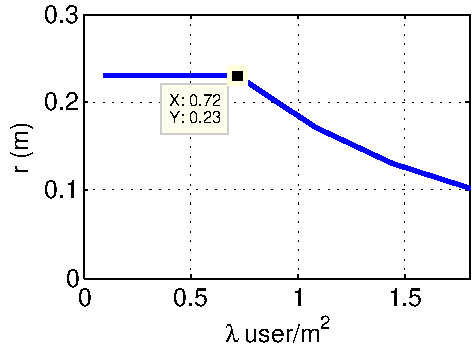
\includegraphics[width = 0.3\textwidth]{Channel_translation_range.pdf}
	\caption{Range of translation $r(\Delta t)$ for different user densities $\lambda$. $r(\Delta t) = 0.23$m for $\lambda<0.72$ and $r = 0.6 \sqrt{1/\lambda\pi}$ for $\lambda >0.72$.}
	\label{fig:Channel_translation_range}
\end{figure}

In Fig. \ref{fig:Channel_sensitivity}, we exhibit the sensitivity of users at different distances. Distant interferers are more sensitive to perturbations than close by interferers. 
This supports the observation that close by users (interferers) will be robust to perturbations and learning the interference from close by neighbors is more reliable. 

\begin{figure}
	\centering
	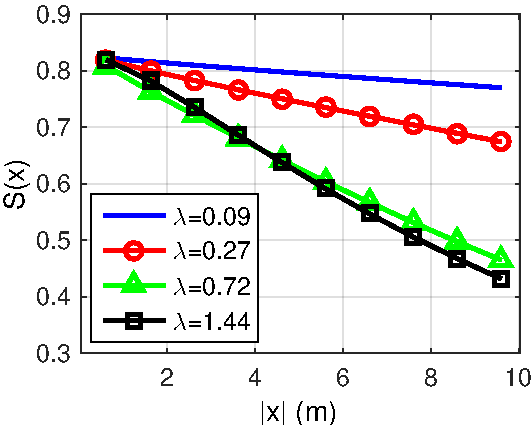
\includegraphics[width = 0.3\textwidth]{Channel_sensitivity.pdf}
	\caption{Sensitivity of users at different distances $|x|$.}
	\label{fig:Channel_sensitivity}
\end{figure}

Fig. \ref{fig:Channel_sensitivity_average} exhibits the average sensitivity of strong interferers $\E[S]$ for different user densities. 
Strong interferers first become more sensitive to movements as $S(x, \Delta t)$ decreases with $\lambda$. 
In highly dense scenarios, strong interferers are closer and the movements become limited, thus the strong interferers become more robust to user local movements.

\begin{figure}
	\centering
	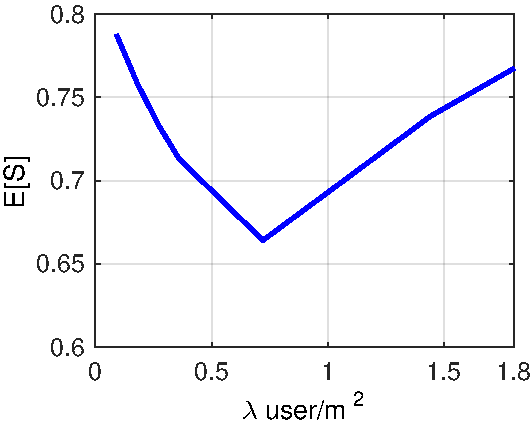
\includegraphics[width = 0.3\textwidth]{Channel_sensitivity_average.pdf}
	\caption{$\mathrm{E}[S(x)|f_0(x_i, \theta_i, \tilde{\Phi}\backslash\{(x_i,\theta_i)\}, \theta_0)=1]$ average sensitivity of strong interferers.}
	\label{fig:Channel_sensitivity_average}
\end{figure}

Our analysis on the number and sensitivity of strong interferers indicate that in dense wearable networks, strong interferers mainly consist of close neighbors and the close neighbors are robust to user movements. The MAC protocol may only need to keep track of and coordinate limited number of close neighbors. Furthermore, users see most strong interferers and most sensitive channels at intermediate densities, thus the design of MAC might be most challenging at intermediate user densities.

\section{Optimizing Clustering in Hierarchical Wearable MAC protocols}\label{section:clustering}
In this section, we discuss how to optimize clustering for hierarchical wearable MAC protocols based on our analysis of interference.

\subsection{Hierarchical MAC for Wearable Networks}\label{section:clustering:hierarchy}
When centralized control is absent, hierarchical clustering and scheduling work as a viable solution to coordinating the multiple PBSSs. 

\begin{figure}
	\centering
	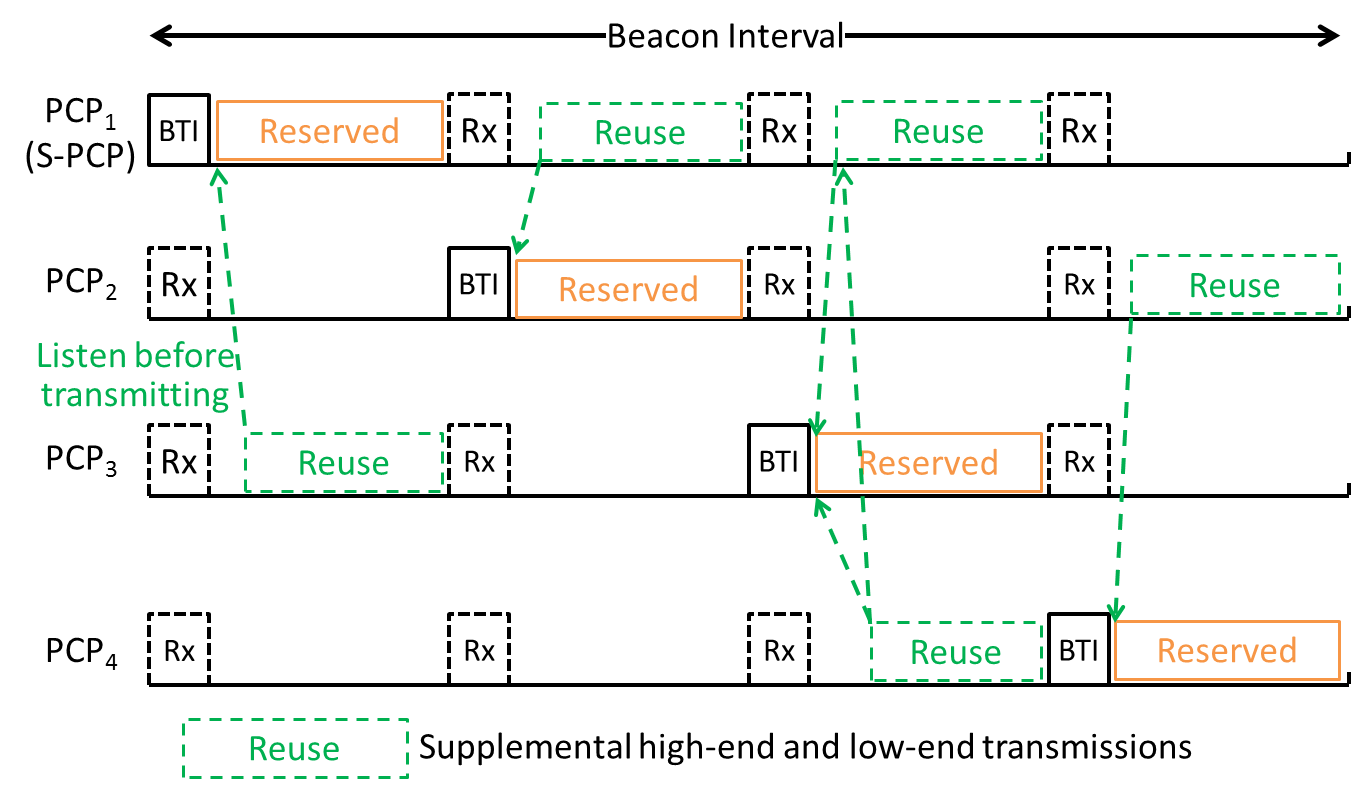
\includegraphics[width = 0.4\textwidth]{Clustering_reuse.pdf}
	\caption{Distributed clustering  with hierarchical scheduling can achieve higher resource reuse and guarantee basic access to channel.}
	\label{fig:clustering:reuse}
\end{figure}

The 802.11ad standard provides a distributed hierarchical MAC geared at coordinating the PBSSs. One PCP is selected as the synchronization PCP (S-PCP) and schedules the transmissions of beacons in the cluster as shown in Fig. \ref{fig:clustering:reuse}. Each PCP is assigned a beacon transmission interval (BTI) to transmit its beacons while other PCPs in the cluster listens to the channel. Problem with the current distributed clustering is that how to form clusters and select channels in dense scenarios is not specified. 
Another problem is that a PBSS may re-schedule its transmissions if it receives the beacon from another PBSSs trying to use the same slots. 
Spatial reuse will be limited, e.g., close to that of time division multiple access (TDMA) if PBSSs within the same cluster can hear each other.

To better serve dense wearable networks, here we discuss the hierarchical protocols consisting of clustering and scheduling based on our analysis of interference. Clustering synchronizes PBSSs and mitigate inter-cluster interference via channel selection, while scheduling aims at improving resource reuse within the cluster. 

The basic principle with clustering is that the channel between the cluster head and cluster members should be strong and stable. 
Another principle is that the cluster members should share a similar set of strong interferers, so that clustering can better mitigate inter-cluster interference.
To meet the above principles, our analysis on channel stability suggest that a cluster should include users in close proximity.

Apart from the problem of what users should be clustered together, an important question is how to choose the proper size for clusters. Many factors influence the best cluster size, e.g., channel quality to cluster head, signaling cost, inter-cluster interference, etc. We try to answer the question by analyzing the resource allocated to each user. 

To achieve better resource reuse within the cluster and meet the basic QoS requirements of each PBSS, a hierarchical scheduling method is used as shown in Fig. \ref{fig:clustering:reuse}. Each PBSS is allocated with some reserved slots where it has higher priority than other PBSSs. Other PBSSs will try to reuse the slots if the their transmissions does not interfere with the transmissions of primary PBSS and contend with other non-primary PBSSs.

\subsection{Modeling Impact of Clustering Size on Achievable Reuse}
In this section we study how cluster size influence the resource available to each PBSS in dense wearable networks where the clustering principles and the hierarchical scheduling are used. 

We use the same system model as Section \ref{section:interference} and consider the performance of PBSSs in a typical cluster. 

The power received at a receiver is given as follows,
\begin{equation*}
P_r = P_t\cdot G_t\cdot G_r \cdot PL.
\end{equation*}
The path loss follows the model in Section \ref{section:interference}. The antennas are directional and the antenna gain follows a 2-D probabilistic model, i.e., 
\begin{equation*}
G = 
\begin{cases}
M, & w.p. ~ \theta/2\pi \\
m, & w.p. ~ 1-\theta/2\pi
\end{cases},
\end{equation*}
where $M$ is the antenna gain of main lobe, $m$ is the antenna gain out of the main lobe, $\theta$ is the beam width.
In each PBSS, there are three types of transmissions with different directionality and transmit power as follows,
\begin{itemize}
	\item Beacon: omni-directional, high power
	\item Primary: directional, high power
	\item Secondary: omni-directional, Low power
\end{itemize}

Assume that clusters are of the same size $K$ and there are $M$ channels. Each cluster include the nearest neighbors of the cluster head and each cluster choose to work on different channels from closest neighbor clusters and the number of users on each channel is equal.
In a typical cluster, the cluster head is located at the center with the $N-1$ cluster members being its closest neighbors.
We assume the cluster members are uniformly distributed on a disc centered at the cluster head with a fixed radius $R_{\mathrm{cluster}}$, see Fig. \ref{fig:clusteranalysis:model}. $R_{\mathrm{cluster}}$ should satisfy that $\lambda \pi (R_{\mathrm{cluster}}^2 - r_{\min}^2) = K - 1$, thus 
\begin{equation*}
R_{\mathrm{cluster}} = \sqrt{\frac{K - 1}{\lambda\pi}+r_{\min}^2}.
\end{equation*}.

Channel selection makes neighboring clusters work on different channels and forms an inter-cluster interference protection region. 
All other PBSSs operating on the same channel, i.e., the inter-cluster interferers, are uniformly distributed outside the protection region, following a HPPP with density $\lambda/M$. On average, there should be $M\cdot K$ users in each cluster's protection region, thus the radius of the region satisfies that 
\begin{equation*}
\lambda \pi (R_{\mathrm{protection}}^2 - r_{\min}^2) = M\cdot K - 1,
\end{equation*}
\begin{equation*}
R_{\mathrm{protect}} = \sqrt{\frac{M\cdot K - 1}{\lambda \pi} + r_{\min}^2}.
\end{equation*}
All users outside the cluster are not synchronized with the cluster and we assume theses users work independently from each other.  

\begin{figure}
	\centering
	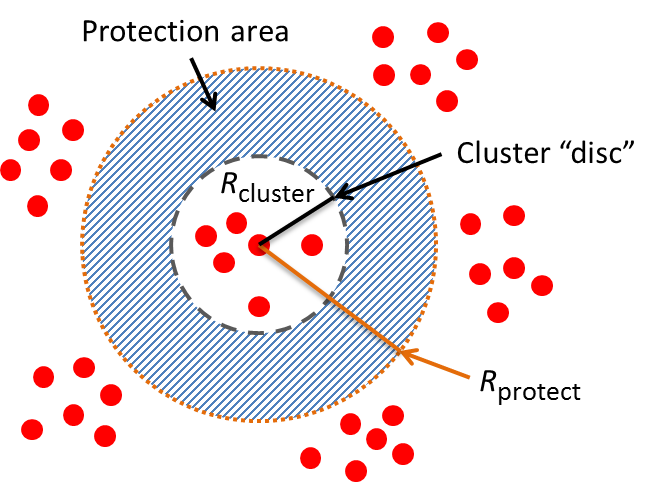
\includegraphics[width = 0.3\textwidth]{Clustering_model.pdf}
	\caption{Model of a typical cluster using clustering and channel selection. Red circles represent users working on the same channel.}
	\label{fig:clusteranalysis:model}
\end{figure}


After modeling clustering, we now introduce the model for scheduling.
There is at most one transmission in each PBSS in each slot. 
Two transmissions interfere with each other if the received power at either receiver exceeds a threshold.

Let $T_{\mathrm{frame}}$ denote the length of frame and $T_{\mathrm{beacon}}$ as the length of one BTI. 
The cluster head reserves exactly $K$ BTIs thus the proportion of data reserved for data transmission is given by
\begin{equation*}
f_{\mathrm{data}} = \frac{T_{\mathrm{data}}}{T_{\mathrm{frame}}}.
\end{equation*}
In each BTI, exactly one PCP will transmit its beacon and the other devices will attempt to receive the beacon using omni-directional mode. 

The PBSSs are full-buffer and schedule primary transmissions in a proportion $\rho_{\mathrm{primary}}\in[0,1]$ of slots for data transmission and schedule secondary transmissions in the remaining $\rho_{\mathrm{secondary}} =1 - \rho_{\mathrm{primary}}$ proportion of the slots. 

We consider two types of scheduling within the cluster, TDMA and hierarchical resource reuse (HRR). In TDMA scheduling, PBSSs share the slots equally within the cluster and the fraction of time that a PBSS can access the channel in a frame is given by, 
\begin{equation*}
p_{\mathrm{access}}^{\mathrm{TDMA}} = f_{\mathrm{data}}/K.
\end{equation*}
A PBSS will schedule primary transmissions in $\rho_{\mathrm{primary}}p_{\mathrm{data}}/K$ slots, and secondary transmissions in $(1-\rho_{\mathrm{primary}})p_{\mathrm{data}}/K$ of the slots. 

In HRR, each PBSS is allocated $1/K$ of the slots where it has higher priority. 
The PBSS first schedules a primary transmission in the reserved slots and schedules other transmissions by reusing the slots allocated to other PBSSs. 
If $\rho_{\mathrm{primary}}\leq 1/K$, the PBSS also schedules secondary transmissions in the allocated slots. 
Other PBSSs would try to reuse the slots if they do not interfere with the user owning the slots.
The probability that a PBSS can reuse the slots in approximated by
\begin{equation*}
\mathrm{P}_{\mathrm{clear}}\cdot \frac{1}{1+\E[N_{\mathrm{intra-cluster}}']},
\end{equation*}
where $\mathrm{P}_{\mathrm{clear}}$ is the probability of not interfering with the primary PBSS, $\E[N_{\mathrm{intra-cluster}}']$ is the expected number of other PBSSs that are trying to reuse the slots and interfering with the reusing PBSS.

A PBSS's transmission is successful if the transmission is not interfered by transmissions outside the cluster. 
Denote by $N_{\mathrm{inter-cluster}}$ as the number of inter-cluster interfering transmissions. 
The activities of inter-cluster interferers are assumed to be mutually independent thus $N_{\mathrm{inter-cluster}}$ follows a Poisson distribution and the probability of a successful transmission can be well approximated as follows, 
\begin{equation*}
p_{\mathrm{success}} = e^{-\E[N_{\mathrm{inter-cluster}}]}.
\end{equation*} 
$N_{\mathrm{intra-cluster}}$ is related to the transmission patterns of PBSSs, which in turn depends on the location of PBSSs within the cluster. 
We use the transmission pattern of a user $\sqrt{2}R_{\mathrm{cluster}}$ away from the cluster head as the typical transmission pattern.

Based on the above analysis, we can evaluate the throughput of a PBSS using the average successful transmission time (STT) of the user,
\begin{equation*}
STT = p_{\mathrm{data}}\times p_{\mathrm{access}} \times p_{\mathrm{success}}.
\end{equation*}

\%Validation of mathematical model

\subsection{Numerical Results and Discussion}
In this section, we compute the STT for different scenarios and characterize the cluster size that maximizes the sum STT of users. 
The parameters used in our analysis are listed in Table \ref{tab:clusteranalysis:parameter}.

\begin{table}
	\centering
	\caption{The parameters used for numerical analysis}
	\begin{tabular}{cc}
		\hline
		Parameter & Value \\
		\hline
		M & 4 \\
		$h_{\mathrm{ceiling}}$ & 2.8 m \\
		$\Gamma_{\mathrm{ceilin}}$ & 0.4654 \\
		$\lambda$ & 1 $\mathrm{user/m^2}$ \\
		$P_t^{\mathrm{high}}$ & 10 dBm \\
		$P_t^{\mathrm{low}}$ & 4 dBm \\
		$P_{\mathrm{threshold}}$ & -78 dBm \\
		$\rho_{\mathrm{primary}}$ & 0.5 \\
		$M_t$,$M_r$ ($\theta = 60\degree$) & 5 dB \\
		$m_t$,$m_r$ ($\theta = 60\degree$) & -5 dB \\
		$M_t$,$M_r$ ($\theta = 24\degree$) & 10 dB \\
		$m_t$,$m_r$ ($\theta = 24\degree$) & -10 dB \\		
		$T_{\mathrm{frame}}$ & 100 ms \\
		$T_{\mathrm{beacon}}$ & 2 ms \\
		\hline
	\end{tabular}
	\label{tab:clusteranalysis:parameter}	
\end{table}
% SINR not considered thus don't need noise figure ? 

In Fig. \ref{fig:clusteranalysis:basic} we show how $STT$ and $p_{\mathrm{success}}$ vary with cluster size for the user located at the center of the cluster.  
$p_{\mathrm{success}}$ increases with $K$ while $p_{\mathrm{data}}$ and $p_{\mathrm{access}}$ decrease. 
STT first increases with $K$, then saturates and decreases, indicating that while large clusters may provide good inter-cluster interference mitigation, they increase the contention between users within the same cluster as well as signaling overheads. 
The STT of primary transmissions is maximized when cluster size is small while the STT of secondary transmissions is maximized for larger $K$, showing that secondary transmissions benefit more from interference mitigation of larger clusters.

\begin{figure}[htp]
	\centering
	\subfloat[Successful transmission time (STT)]{\label{subfig:basic_stt}\includegraphics[width=0.3\textwidth]{Cluster_analysis_basic_stt.pdf} } \hfill
	
	\subfloat[Probability of successful transmission $p_{\mathrm{success}}$]{\label{subfig:basic_psuccess} \includegraphics[width=0.3\textwidth]{Cluster_analysis_basic_psuccess.pdf}}
	
	\caption[]{STT for data transmission \subref{subfig:basic_stt} and $p_{\mathrm{success}}$ \subref{subfig:basic_psuccess} for different cluster sizes. $\theta=60\degree$, $\rho_{\mathrm{primary}} = 0.5$. }
	\label{fig:clusteranalysis:basic}
\end{figure}

In Fig. \ref{fig:clusteranalysis:directionality} we compare STT when the antennas of primary transmissions have different degrees of directionality. In Fig. \ref{fig:clusteranalysis:primary_ratio} we exhibit the STT when users have different proportions of primary transmissions, $\rho_{\mathrm{primary}}$. 
The optimal cluster size is smaller when transmissions are more directional. 
Results suggest that highly directional devices are less dependent on clustering to mitigate interference, thus users with highly directional devices may favor small clusters or not joining clusters at all. 
\begin{figure}
	\centering
	\includegraphics[width = 0.3\textwidth]{Cluster_analysis_directionality.pdf}
	\caption{STT for antennas with different directionality.}
	\label{fig:clusteranalysis:directionality}
\end{figure}

\begin{figure}
	\centering
	\includegraphics[width = 0.3\textwidth]{Cluster_analysis_primary_ratio.pdf}
	\caption{STT for different tranffic patterns $\rho_{\mathrm{primary}}$.}
	\label{fig:clusteranalysis:primary_ratio}
\end{figure}

In Fig. \ref{fig:clustereanalysis:optimal_cluster_size} we show how the cluster size maximizing the STT changes with the user density. 
When user density is high, the optimal cluster size does not change very much, indicating that optimal cluster size are pretty robust to user density. 
However, as we have discussed, the directionality and proportion of different types of traffic influence the optimal cluster size. 

\begin{figure}
	\centering
	\includegraphics[width = 0.3\textwidth]{Cluster_analysis_optimal_cluster_size.pdf}
	\caption{Cluster size that maximizes STT for different user densities.}
	\label{fig:clustereanalysis:optimal_cluster_size}
\end{figure}

In Fig. \ref{fig:clusteranalysis:compare_mac} we compare the STT for different MAC protocols for different user densities. 
At each user density, the cluster size is chosen as the one that maximizes the total STT. 
For Aloha, users select channels randomly and the access probability is optimized to maximize the total STT. 
Our first observation is that clustering and reuse provide moderate gain in STT, partly due to beacon overheads, but improves the probability of successful transmission. 
Our second observation is that the total STT first decreases with user density then starts to increase with density. 
Such a result is in line with our analysis of the interference environment that in very dense networks, close by neighbors block the interference from distant interferers thus the interference in dense environments may not be the worst case. 
Our observation comes from the MAC perspective, and in fact sum interference will keep increasing with user density if no MAC scheduling or simple ALOHA is used, although the rate of increase becomes smaller at high user densities. 

\begin{figure}
	\centering
	\includegraphics[width = 0.3\textwidth]{Cluster_analysis_compare_mac.pdf}
	\caption{Sum STT in different user densities for different MAC protocols, optimal Aloha, Cluster + TDMA and Cluster + IRR.}
	\label{fig:clusteranalysis:compare_mac}
\end{figure}

%Conclusion for analysis of clusters?

\section{Conclusion}\label{section:conclusion}
Our analysis of strong interferers shows that enabling mmWave wearable networks in high user densities does seem feasible from MAC design perspective. 
Blockage and directionality help limit the number of strong interferers to a few that are close by. 
PBSSs may then coordinate with close neighbors through coarse grain coordination at reasonable overheads while treating interference from distant PBSSs as 
noise. 
However, the fast changing nature due to self-blockage and movements still pose challenges on tracking and coordinating of interferers. 
For a relative stationary network, clustering with resource reuse works as a viable solution to coordinating the PBSSs. 
Finding the optimal cluster size requires trade-off between interference mitigation and resource reuse within cluster thus an ideal cluster protocol should adapt to different environment. 
When users are highly mobile, the channel changes very quickly and it is hard to maintain the cluster thus the PBSSs may just work on its own instead of joining clusters. 

\begin{thebibliography}{50}
\bibitem{wearable}
``Smart Wearable Devices: Fitness, Glasses, Watches, Multimedia, Clothing, Jewellery, Healthcare \& Enterprise 2014-2019,'' \emph{Juniper Research}, Aug. 2014.

\bibitem{80211ad}
\emph{``IEEE Standard for Information Technology — Telecommunications and Information Exchange between Systems — Local and Metropolitan Area Networks — Specific Requirements. Part 11: Wireless MAN Medium Access Control (MAC) and Physical Layer (PHY) Specifications Amendment 3: Enhancements for Very High Throughput in 60 GHz Band,''}, IEEE Standard 802.11ad, 2012.

\bibitem{802153c}
\emph{``IEEE Standard for Information Technology — Telecommunications and Information Exchange between Systems — Local and Metropolitan Area Networks — Specific Requirements. Part 15.3: Wireless Medium Access Control (MAC) and Physical Layer (PHY) Specifications for High Rate Wireless Personal Area Networks (WPANs) Amendment 2: Millimeter-Wave-Based Alternative Physical Layer Extension,''} IEEE Std 802.15.3c, 2009.

\bibitem{ECMA387}
\emph{``High Rate 60 GHz PHY, MAC and PALs,''} ECMA Standard 387, 2010.

%\bibitem{mmwave_propagation}
%S. Y. Geng, J. Kivinen, X. W. Zhao, and P. Vainikainen, ``Millimeter-wave propagation channel characterization for short-range wireless communications,'' \emph{IEEE Trans. Veh. Tachnol.}, vol. 58, no. 1, pp. 3-13, Jan. 2009.

\bibitem{humanshadowing}
C. Gustafson and F. Tufvesson, \emph{``Characterization of 60 GHz Shadowing by Human Bodies and Simple Phantoms, ''} Antennas and Propagation (EUCAP), 6th European Conference on, 2012.

\bibitem{urbanblockage}
T. Bai and R.W. Heath Jr., ``Coverage and rate analysis for millimeter wave cellular networks,'' in \emph{IEEE Trans. Wireless Comm.}, vol. 13, no. 9, Sep. 2014.

\bibitem{interferencefinitesized}
K. Venugopal, M.C. Valenti and R.W. Heath, \emph{``Interference in Finite-Sized Highly Dense Millimeter Wave Networks,''} Information Theory and Applications Workshop, Feb. 2015.

\bibitem{enclosedmmwave}
G. George and A. Lozano, ``Performance of enclosed mmWave wearable networks,'' in IEEE Int'l Workshop on Compuational Advances in Multi-Sensor Adaptive Processing (CAMSAP 15), Dec. 2015. (Revision required)

\bibitem{humanactivity}
S. Collonge, G. Zaharia and G.E. Zein, ``Influence of human activity on wide-band characteristics of the 60 GHz indoor radio channel,'' \emph{IEEE Trans. Wirel. Commun.}, vol. 3,  no. 6, pp. 2369-2406, 2004.

\bibitem{timevaryingpathshadowing}
I. Kashiwagi, T. Taga and T. Imai, ``Time-varying path-shadowing model for indoor populated environments,'' \emph{IEEE Trans. Veh. Technol.}, vol. 59, no. 1, Jan. 2010.

\bibitem{blockagein60ghz}
S. Singh, F. Ziliotto, U. Madhow, E. M. Belding and M. Rodwell, ``Blockage and Directivity in 60 GHz Wireless Personal Area Networks: From Cross-Layer Model to Multihop MAC Design,'' \emph{IEEE J. Sel. Areas Commun.}, vol. 27, no. 8, Oct. 2009.

%\bibitem{virtualtimeslot}
%C. Sum, Z. Lan, R. Funada, J. Wang, T. Baykas, M. A. Rahman, and H. Harada, ``Virtual time-slot allocation scheme for throughput enhancement in a millimeter-wave multi-Gbps WPAN system,'' \emph{IEEE J. Sel. Areas Commun.}, vol. 27, no. 8, Oct. 2009.

%\bibitem{rex}
%L. X. Cai, L. Cai, X. Shen, and J. Mark, ``REX: a randomized exclusive region based scheduling scheme for mmWave WPANs with directional antenna,'' \emph{IEEE Trans Wireless Commun.}, vol. 9, no. 1, pp. 113-121, Jan. 2010. 

%\bibitem{fdmac}
%I. K. Son, S. Mao, M. X. Gong, and Y. Li, ``On frame-based scheduling for directional mmWave WPANs,'' in \emph{Proc. IEEE INFOCOM}, Orlando, FL, 2012, pp. 2149-2157.

\bibitem{dtdmac}
E. Shihab, L. Cai, and J. Pan, ``A distributed asynchronous directional-to-directional MAC protocol for wireless ad hoc networks,'' \emph{IEEE Tans. Veh. Tech.}, vol. 58, no. 9, pp. 5124-5134, Nov. 2009. 

\bibitem{mdmac}
S. Singh, R. Mudumbai, and U. Madhow, ``Distributed coordination with deaf neighbors: efficient medium access for 60 GHz mesh networks,'' in \emph{Proc. IEEE INFOCOM}, San Diego, CA, 2010, pp. 1-9.

\bibitem{onlinkscheduling}
Z. He, S. Mao and T.S. Rappaport, \emph{``On Link Scheduling Under Blockage and Interference in 60-GHz Ad Hoc Networks,''} edition required...

\bibitem{intersharing}
W. Feng, Y. Li, D. Jin and L. Zeng, \emph{``Inter-Network Spatial Sharing with Interference Mitigation Based on IEEE 802.11ad WLAN System,''} Globecom 2014 workshop - telecommunications standards - from research to standards


%\bibitem{mmwaveadhoc}
%A. Thornburg, T. Bai and R.W. Heath Jr., ``Interference statistics in a random mmWave ad hoc network,'' in IEEE Int'l Conference on Acoustics, Speech and Signal Processing (ICASSP), Apr. 2015.

\bibitem{reflection}
K. Sato \emph{et al.}, ``Measurements of Reflection and Transmission Characteristics of Interior Structure of Office Building in the 60-GHz band,'' \emph{IEEE Trans. Antennas Propag.}, vol. 45, no. 12, pp. 1783-1792, Dec. 1997.

\bibitem{stochasticgeometry}
F. Baccelli and B. Blaszczyszyn, ``Stochastic geometry and wireless networks, volume \Rom{1} - theory,'' \emph{Foundations and Trends in Networking}, vol. 3, no. 3-4, pp. 249-449, 2009.

\bibitem{poisson}
J. F. C. Kingman, ``Poisson Processes,'' New York: The Clarendon Press Oxford Univ. Press, 1993.

\bibitem{stochasticapp}
S.N. Chiu, D. Stoyan, W.S. Kendall and J. Mecke, \emph{Stochastic Geometry and its Applications} (3rd ed). Hoboken: Wiley, 2013. 

\bibitem{busyperiod_heavytraffic}
P. Hall, ``Heavy Traffic Approximations for Busy Period in an M/G/$\infty$ Queue,'' \emph{Stochastic Processes and their Applications}, vol. 19, no. 2, pp. 259-269, 1985.

\bibitem{busyperiod_exponential}
M. A. M. Ferreira and M. Andrade, ``The M/G/$\infty$ Queue Busy Period Distribution Exponentiality,'' \emph{Applimat - Journal of Applied Mathematics}, vol. 4, no. 3, pp. 249-260, 2011.


\bibitem{matern}
B. Mat\'ern, Spatial Variation second ed. vol.36 of Lecture Notes in Statistics. (Revision required)

%\bibitem{backoff}
%H. Lee, H. Kwon, A. Motskin and  L. Guibas, \emph{``Interference-aware MAC Protocol for Wireless Networks by a Game-Theoretic Approach,''}, in \emph{INFOCOM}, Rio de Janeiro, 2009, pp. 1854-1862.

%\bibitem{apcluster}
%B.J. Frey and D. Dueck, \emph{``Clustering by Passing Messages Between Data Points,''} Science 315 (2007) 972-976.

%\bibitem{apvanet}
%B. Hassanabadi, C. Shea, L. Zhang and S. Valaee, \emph{``Clustering in Vehicular Ad Hoc Networks using Affinity Propagation,''} Ad Hoc Networks 13 (2014) 535-548.

%\bibitem{apd2d}
%D.J. Son, C.H. Yu and D.I Kim, \emph{``Resource Allocation based on Clustering for D2D Communications in Underlaying Cellular Networks,''} in \emph{Information and Communication Technology Convergence}, Busan, 2014, pp. 232-237.


%\bibitem{cocurrentbf}
%J. Qiao, X. Shen, J.W. Mark and Y. He, \emph{``MAC-layer Concurrent Beamforming Protocol for Indoor Millimeter Wave Networks''}, in \emph{IEEE Trans. Veh. Tachnol.}, vol , no. ,   2014. 

\end{thebibliography}

\end{document}
